\section{Simulations}

\subsection{Rotating ball in zero gravity}

\begin{wrapfigure}{R}{0.45\linewidth}
    \centering
    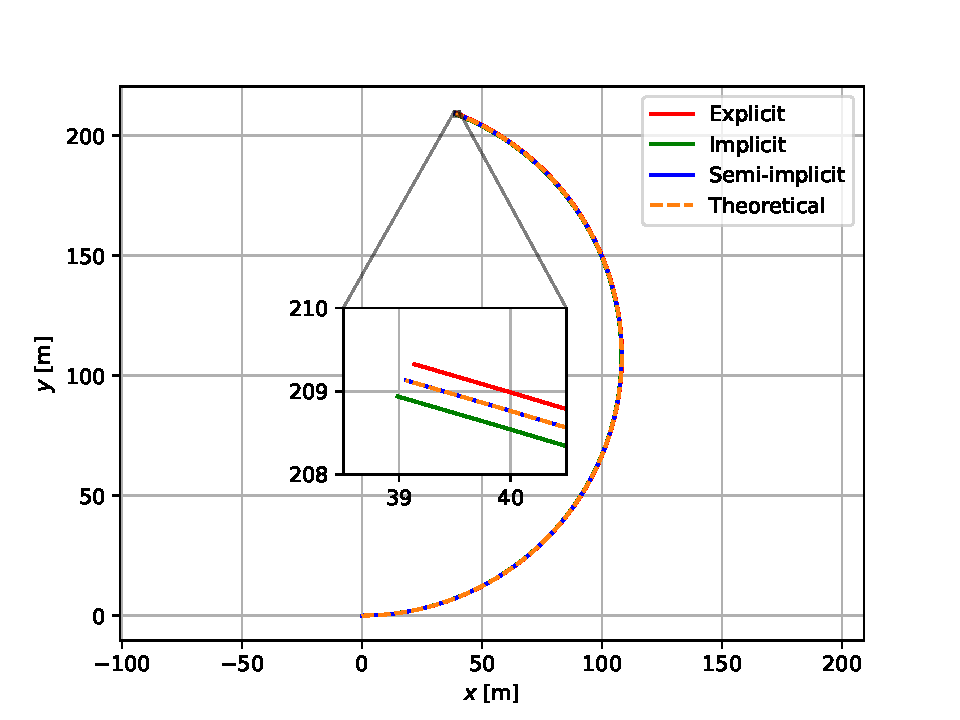
\includegraphics[width=0.85\linewidth]{figures/nograv_trajectory_all.pdf}
    \caption{Postion of the ball after $t_\textrm{fin}$ for different methods ($n_\textrm{steps} = 2000$)}
    \label{fig:nograv:trajectory_all}
    \vspace*{-1cm}
\end{wrapfigure}
The simulations were done on a tenis ball of mass $m = 0.056$ kg and radius $R = 0.033$ m, with air density $\rho = 1.2$ kg/m$^3$. The coefficient $\mu = 6$ has been chosen. The ball is sent with initial conditions $\omega = 10$ rotations/s ($\omega = 20\pi$ rad/s), $\vec{x}(0) = \vec{0}$, $\vec{v}(0) = 5 \vec{e_x}$ m/s and its trajectory is simulated until \mbox{$t_\textrm{fin} = 60$ s}.

To lighten the notation, we will use EE for the Explicit Euler method, IE for Implicit Euler and SE for Semi-implicit Euler.

The position after $t_\textrm{fin}$ is shown in \autoref{fig:nograv:trajectory_all}. We can see that the EE method overshoots the expected trajectory, while the IE method undershoots it and SE remains almost exactly on the analytical result.


\subsubsection{Numerical convergence}

The numerical convergence of the final position of each method is illustrated in \autoref{fig:nograv:convergence}. We observe that the error on the final position tends to 0 as $\Delta t \rightarrow 0$ for every method, meaning that they all converge numerically. Furthermore, the order of convergence is given by the slope of the line passing through the points. We can thus deduce that the order of convergence is 1 for EE and IE, and 2 for SE.

\begin{figure}[h]
    \centering
    \begin{subfigure}{0.45\linewidth}
        \centering
        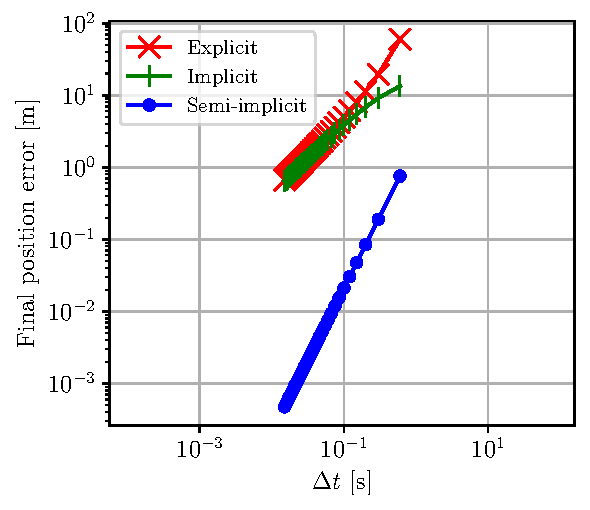
\includegraphics[width=\linewidth]{figures/nograv_numeric_convergence_all.pdf}
        \caption{Error on final position w.r.t. analytical solution. $n_\textrm{steps}$ was varied between 100 and 4000.}
        \label{fig:nograv:convergence}
    \end{subfigure}
    \hspace*{0.2cm}
    \begin{subfigure}{0.45\linewidth}
        \centering
        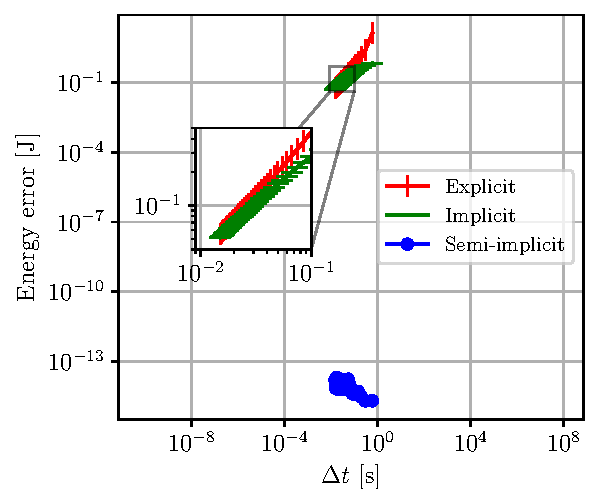
\includegraphics[width=\linewidth]{figures/nograv_energy_error_all.pdf}
        \caption{Error on final energy for each method where the error is defined as $\max(E_\textrm{mec}) - \min(E_\textrm{mec}).$ (maximum $n_\textrm{steps}=4000$)}
        \label{fig:nograv:energy_error}
    \end{subfigure}
    \caption{Numerical convergence analysis for different methods}
\end{figure}

The numerical convergence of the energy for each method is also given in \autoref{fig:nograv:energy_error}. Again, we observe that the error clearly tends to 0, as $\Delta t \rightarrow 0$ for EE and IE. The error for SE remains quite constant and is of the order of $10^{-14}$, close to the limit for double-precision floating point numbers. We thus conclude that every method converges numerically. The order of convergence for EE and IE is 1, but SE does not have an order of convergence for the energy as it remains pretty much constant for a wide range of $\Delta t$.

\subsubsection{Numerical stability}

To illustrate the numerical stabilty of each method, the energy over time has been plotted in \autoref{fig:nograv:energy}. EE is numerically unstable, as its energy over time grows exponentially for smaller $n_\textrm{steps}$. IE is stable, but loses energy over time, decaying exponentially. Using a curve fit of the function $g(t) = A + e^{\gamma t}$, where A is an offset and $\gamma$ is the growth rate, we obtain the values of $\gamma$ presented in \autoref{tab:nograv:rate}. This shows that the absolute value of $\gamma$ decreases with $\Delta t$, illustrating the numerical convergence. Finally, the SE method remains at constant energy even for smaller $n_\textrm{steps}$, meaning it is both stable and conserves energy.

\begin{figure}[h]
    \centering
    \begin{subfigure}{0.5\linewidth}
        \centering
        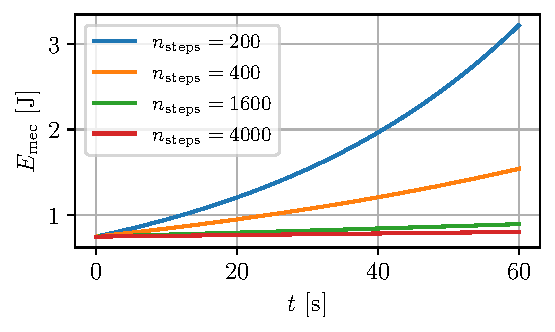
\includegraphics[width=\linewidth]{figures/nograv_energy_explicit.pdf}
        \caption{Explicit}
    \end{subfigure}%
    \begin{subfigure}{0.5\linewidth}
        \centering
        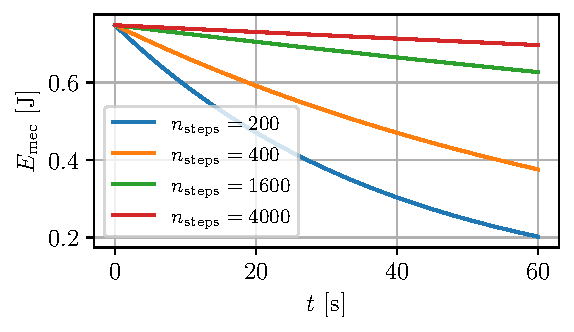
\includegraphics[width=\linewidth]{figures/nograv_energy_implicit.pdf}
        \caption{Implicit}
    \end{subfigure}
    \begin{subfigure}{0.6\linewidth}
        \centering
        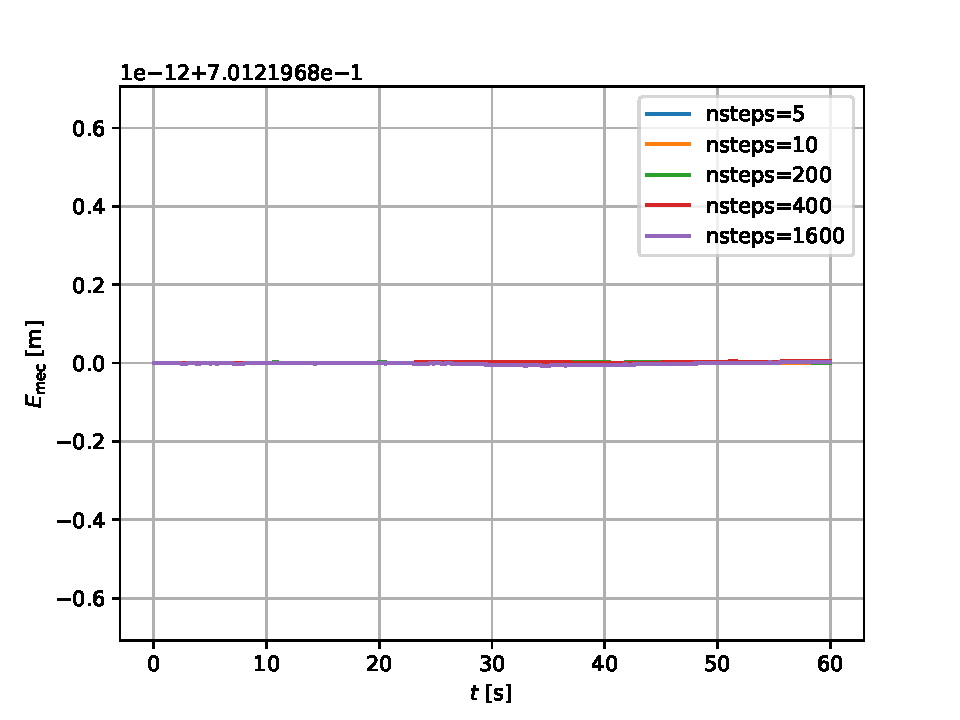
\includegraphics[width=\linewidth]{figures/nograv_energy_semiimplicit.pdf}
        \caption{Semi-implicit}
    \end{subfigure}
    \caption{Energy over time for different methods and $n_\textrm{steps}$. To improve the results, the tolerance on the error was set to $10^{-10}$}
    \label{fig:nograv:energy}
\end{figure}

\begin{table}[h]
    \centering
    \begin{tabulary}{0.8\linewidth}{C|C|C|C|C}
        \toprule
        $n_\textrm{steps}$ & 200 & 400 & 1600 & 4000 \\
        \midrule
        EE & 0.0203 & 0.0096 & 0.0023 & 0.0009 \\
        IE & -0.0146 & -0.0081 & -0.0022 & -0.0009 \\
        \bottomrule
    \end{tabulary}
    \caption{Rate of growth or decrease of the energy for non energy-conserving methods}
    \label{tab:nograv:rate}
\end{table}

\subsection{Rotating ball with gravity}

\subsubsection{Method comparison}
\label{seq:gravrot:comp}

\begin{figure}[h]
    \centering
    \begin{subfigure}{0.49\linewidth}
        \centering
        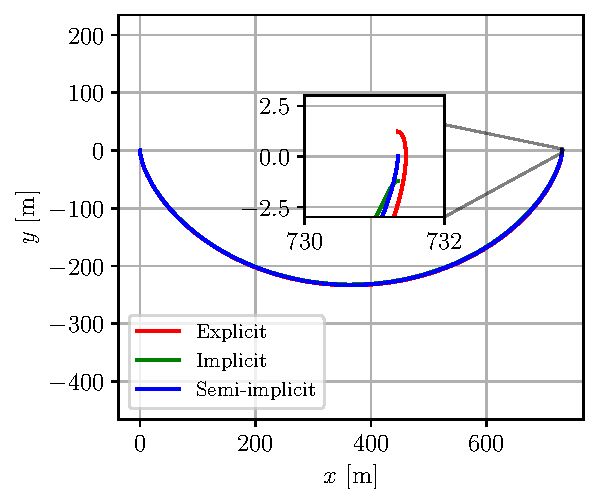
\includegraphics[width=\linewidth]{figures/rotate_grav_trajectories.pdf}
        \caption{Trajectories of the falling ball with each method}
        \label{fig:rotate_grav:traj}
    \end{subfigure}
    \hspace*{0.2cm}
    \begin{subfigure}{0.47\linewidth}
        \centering
        
\includegraphics[width=\linewidth]{figures/rotate_grav_energy.pdf}
        \caption{Evolution of the energy of the simulation for each method}
        \label{fig:rotate_grav:nrj}
    \end{subfigure}
    \caption{Simulation of the falling tennis ball with the three methods EE, IE and SE \mbox{($n_\textrm{steps}=2000$)}}
\end{figure}

Another set of simulations was run with $\vec{g} = -9.81 \vec{e}_y$ m/s$^2$ to analyse a more realistic trajectory. The tenis ball is let go at $\vec{x}(0) = \vec{0}$ and with $\vec{v}(0) = \vec{0}$. It rotates with the same angular speed $\omega$ as in the previous part. The simulation was run up to the time $t_\mathrm{fin}$ calculted in \ref{seq:analytics_gravity} for the numerical values given. The given results for trajectories and energy are shown respectively in \autoref{fig:rotate_grav:traj} and \autoref{fig:rotate_grav:nrj}.

The trajectories obtained are extremely similar and diverge slightly around the end of the simulation as the close-up view shows. The expected behavior is observed with EE slightly overshooting, having gained energy, and IE falling short of reaching the original height of $y(0) = 0$ with a loss of energy. As before, the SE method is extremely precise, ending up exactly at the expected height at the time of the end of the simulation corresponding to the theoretical value.

In particular the \autoref{fig:rotate_grav:nrj} shows the great stability of the SE method with an energy seemingly constant. The EE and IE do not conserve energy with the energies diverging from the theoretically constant value. For EE this results in unstability with a growing energy. For IE the energy diminishes making this method non-energy conserving but still stable. This can be illustrated by observing the trajectories for larger times as shown in \autoref{fig:rotate_grav:yolo} with \mbox{$t_\mathrm{fin} = 300$ s}. In this new simulation it is obvious that the EE diverges strongly. Observing the IE it can also be seen that the amplitude of its oscillations diminish through time as it loses energy.

\begin{figure}[H]
    \centering
    \begin{minipage}{.47\linewidth}
        \centering
        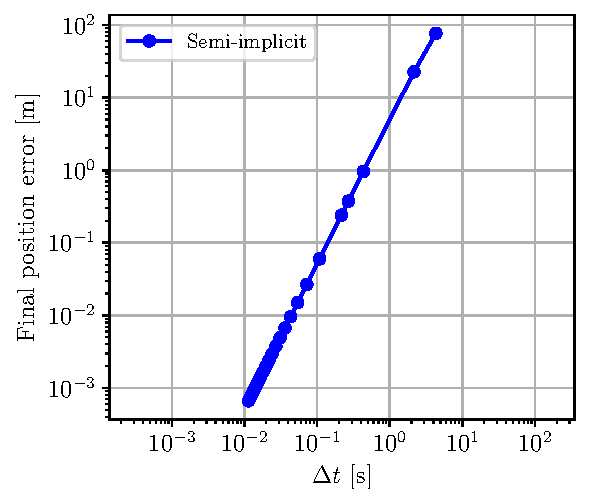
\includegraphics[width=\linewidth]{figures/rotate_grav_errors.pdf}
        \caption{Error on the final position after one oscillation ($t_\mathrm{fin} \approx 21.6$ s) for the falling ball}
        \label{fig:rotate_grav:errors}
    \end{minipage}
    \hspace*{0.2cm}
    \begin{minipage}{.49\linewidth}
        \centering
        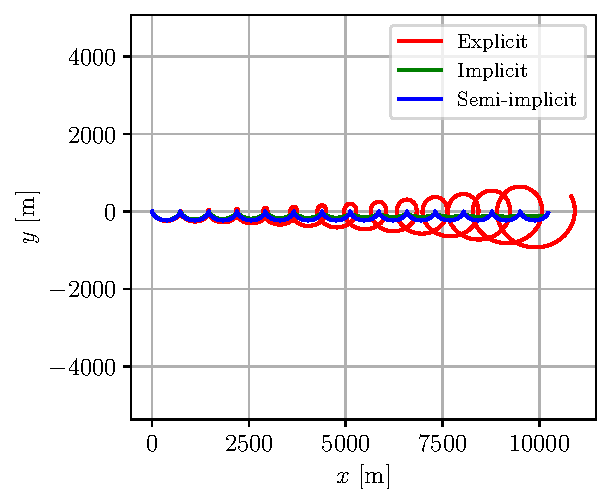
\includegraphics[width=\linewidth]{figures/rotate_grav_trajectories_yolo.pdf}
        \caption{Trajectories for the falling tennis ball with each method for $t_\mathrm{fin} = 300$ s}
        \label{fig:rotate_grav:yolo}
    \end{minipage}
\end{figure}

The SE method as been shown to give better results than the other two in this simulation as well. It can also be of interest to determine its order of convergence. As shown in \autoref{fig:rotate_grav:errors} the error tends to $0$ as $\Delta t \rightarrow 0$ meaning this method converges numerically. The figure is represented with a log-log scale which allows to read the order of convergence for the SE method is 2.

\subsubsection{Adding drag force}

The aerodynamic drag force
\be
    \vec{F_t} = -\frac{1}{2}C_t \rho S \|v\| \vec{v}
\ee
was added to the simulation by adding a term to $f(\textbf{y})$ from \autoref{eq:ode}
\be
    f(\textbf{y}) = \left(\begin{matrix}
    v_x \\
    v_y \\
    -\frac{\mu R^3 \rho \omega}{m} v_y  - \frac{1}{2m} C_t \rho S \|v\| v_x \\
    \frac{\mu R^3 \rho \omega}{m} v_x - g - \frac{1}{2m} C_t \rho S \|v\| v_y
    \end{matrix}\right)
\ee

In order to simulate this system, the SE method was used as it yields better results than EE or IE. The parameters of the simulation were as described in \ref{seq:gravrot:comp} and with $C_t = 0.35$, $S = \pi R^2$.

The trajectory is shown in \autoref{fig:gravfrict:pos} and seems to behave as expected, with an equilibrium between the applied forces of the air drag, the Magnus effect and the weight that make it follow a straight path. As shown in \autoref{fig:gravfrict:conv}, the order of convergence of the final position is 2.

\begin{figure}[h]
    \centering
    \begin{subfigure}{0.49\linewidth}
        \centering
        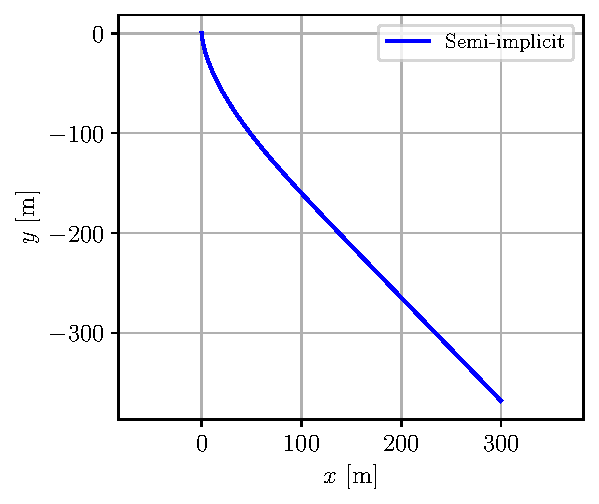
\includegraphics[width=\linewidth]{figures/grav_frict_position.pdf}
        \caption{Trajectory after $t_\textrm{fin}$ ($n_\textrm{steps}=4000$)}
        \label{fig:gravfrict:pos}
    \end{subfigure}%
    \hspace*{0.2cm}
    \begin{subfigure}{0.45\linewidth}
        \begin{subfigure}{\linewidth}
            \centering
            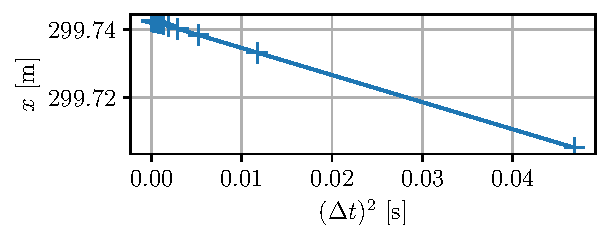
\includegraphics[width=\linewidth]{figures/grav_frict_convergence_x.pdf}
        \end{subfigure}
        \begin{subfigure}{\linewidth}
            \centering
            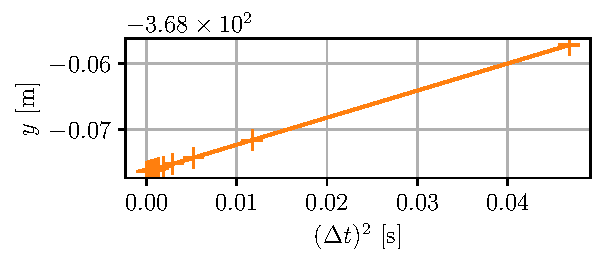
\includegraphics[width=\linewidth]{figures/grav_frict_convergence_y.pdf}
        \end{subfigure}
        \caption{Convergence analysis for the final position. $n_\textrm{steps}$ was varied between 100 and 4000.}
        \label{fig:gravfrict:conv}
    \end{subfigure}
    \caption{Simulation of the system including air drag using the SE method}
\end{figure}

